% 第 3 章 弱网自治场景
\chapter{弱网自治场景}

弱网自治是 EdgeFlow 面向矿区、海上平台、偏远园区等网络不稳定环境的核心理念：\textbf{断网业务不中断、恢复后自动对账}。本章描述三层自治设计、特性引用、参数调优与验证演练。

\section{业务痛点}

\begin{itemize}
  \item \textbf{断网业务中断}：依赖云端协同的采集与控制业务在断网时停摆，现场生产受影响。
  \item \textbf{恢复后状态不一致}：断网期间边缘持续运行产生状态漂移，恢复后云端与边缘不一致，需人工对账。
  \item \textbf{命令丢失}：弱网抖动造成下行指令丢失或重复，设备状态不可预期。
  \item \textbf{运维被动}：节点离线发现滞后，恢复依赖人工干预，长周期弱网场景缺乏保障手段。
\end{itemize}

\section{方案设计}

三层自治设计：

\textbf{业务自治——容器持续运行与自愈。} 断网期间 Pod 容器持续运行：Edged 以 5s 周期本地调谐（F11），期望态持久化于 SQLite（F17）；本地设备指令（MQTT command 主题）照常下发；影子持续更新，op-ledger 照常落 SQLite；Pod/Config 期望态边缘持久，不依赖云端补发。

\textbf{数据自治——状态快照 + 周期补报（如实口径）。} 断网期间采集完全不受影响（2s 采样循环与网络无关，Modbus 本地直连照常）；DeviceReport 发送失败仅记 Warn，不缓存、不重试、不落盘，内存影子持续更新。恢复后无全量/增量同步协议，靠下一轮周期上报（$\le$30s）补报\textbf{最新状态快照}——即“状态级断点续传”，\textbf{不支持历史遥测样本回补}（断网期间样本不落盘）。业务需要历史留存时，应在 EventBus 侧或应用侧自行订阅持久化。

\textbf{通道自治——退避重连 + 可靠投递 + 幂等。} 云边通道断线后指数退避重连（1s 起步、翻倍、封顶 60s，注册成功重置，F04）；下发消息可靠投递（pending+Ack、同 ID 重发、最多 3 次尝试、超时 504，F05）；边缘侧幂等去重（同 ID 缓存 1000 条 FIFO，F05），重发不重复执行；重连后第一条消息永远是 Register（每次连接重新注册，F02），随后周期上报自动重建云端视图。

\section{产品特性引用}

\textbf{表 3-1：弱网自治场景特性引用}

{\small\setlength{\tabcolsep}{3pt}
\begin{tabular}{@{}p{1.6cm}p{0.8cm}p{6.6cm}p{5.6cm}@{}}
\toprule
弱网环节 & 特性 & 能力说明 & 弱网价值\\
\midrule
云边通道 & F01 & WebSocket 云边管理面通道（TLS 开启自动升级 wss） & 一条连接承载全部控制与状态消息\\
节点注册 & F02 & 连接建立后首条消息 Register，RegisterAck 超时 10s & 重连即重新注册，身份自动恢复\\
心跳保活 & F03 & 30s 周期心跳 & 通道活性探测，支撑离线判定\\
退避重连 & F04 & 断线后 1s 起步翻倍、封顶 60s、注册成功重置 & 避免重连风暴，弱网抖动自动恢复\\
可靠投递 & F05 & pending+Ack、同 ID 重发、最多 3 次尝试、幂等去重 1000 条、超时 504 & 下发指令不丢不重，弱网可靠闭环\\
节点在线/离线判定 & F07 & CloudHub 90s 断开 + NodeController 180s 心跳停滞（扫描 30s）双路径 & 离线判定不悬挂，状态最终收敛\\
节点状态语义 & F08 & Ready/Unknown/Offline 三态 & 状态标准化，与 K8s 语义对齐\\
云端状态自愈 & F09 & 云端分级持久化（v0.4.0 起）：注册台账与 Desired 跨重启保留，边缘重连自动重注册恢复 & 云端重启无需人工恢复\\
声明式调谐 & F11 & 5s 周期本地对账，期望态在 SQLite & 断网期间容器持续收敛，业务不中断\\
多副本 & F12 & replicas 补齐/收缩 & 单副本异常自动补齐\\
健康自愈 & F13 & Inspect 非 Running 自动重启 & 容器异常自动恢复，无需人工\\
CrashLoopBackOff & F14 & 3 次阈值/30s 退避/60s 稳定重置 & 崩溃循环自动退避，保护节点资源\\
镜像漂移检测 & F15 & 期望镜像比对、漂移重建（批 1 滚动） & 镜像被篡改自动还原，防漂移\\
断网自治 & F16 & 云端不可达容器持续运行，恢复自动同步 & 断网业务不中断（E2E 60s 实测）\\
MetaManager 持久化 & F17 & SQLite（WAL）落盘元数据/Pod/配置 & 期望态不丢，重启按声明收敛\\
PodStatus 上报 & F18 & 30s 周期（可配 1s--10min），Absent 终态保留 90s & 云端实时掌握 Pod 运行状态\\
增量订阅通知 & F20 & MetaManager 本地变更订阅通知 & 边缘模块解耦联动\\
\bottomrule
\end{tabular}}

\section{部署方式}

\begin{figure}[htbp]
  \centering
  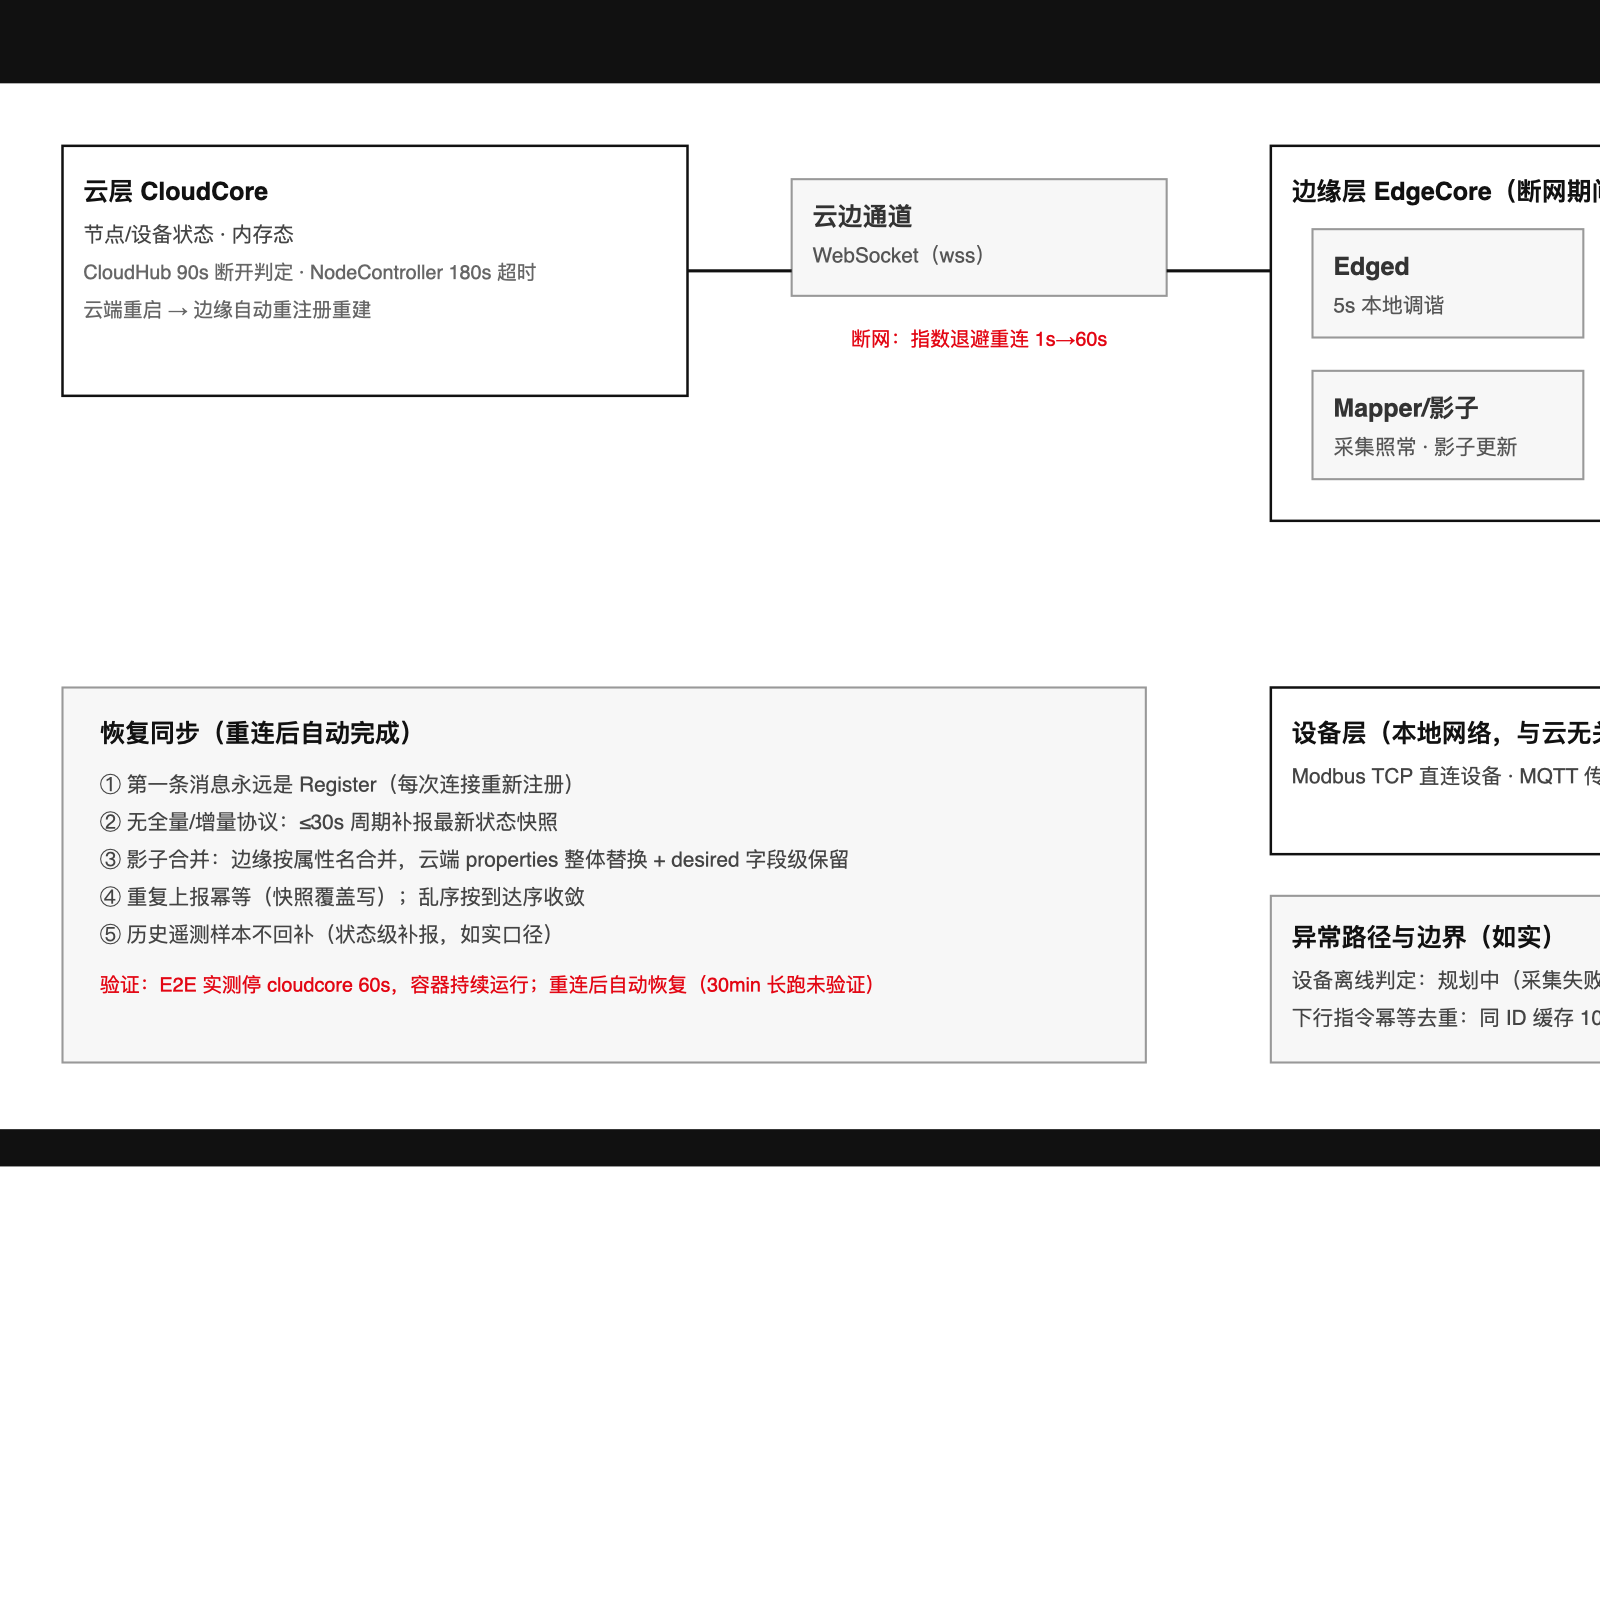
\includegraphics[width=0.94\textwidth]{../diagrams/scenario-weaknet.png}
  \caption{弱网自治场景部署拓扑}
  \label{fig:weaknet}
\end{figure}

\textbf{弱网参数调优（env）}：

\textbf{表 3-2：弱网参数调优}

{\small\setlength{\tabcolsep}{3pt}
\begin{tabular}{@{}p{5.2cm}p{2.4cm}p{8.2cm}@{}}
\toprule
参数 & 默认 & 说明\\
\midrule
云边心跳周期 & 30s & 通道活性探测间隔（F03）\\
退避重连上限 & 60s & 断线重连指数退避封顶（F04）\\
\env{EDGEFLOW\_EDGECORE\_DEVICE\_REPORT\_INTERVAL} & 30s（1s--10min） & 设备状态上报周期，弱网可调大降低流量（F22）；\textbf{支持热重载}\\
\env{EDGEFLOW\_EDGECORE\_REPORT\_INTERVAL} & 30s（1s--10min） & Pod 状态上报周期（F18）；\textbf{支持热重载}\\
\env{EDGEFLOW\_CLOUDCORE\_NODE\_SCAN\_INTERVAL}/\env{NODE\_TIMEOUT} & 30s / 180s & 节点心跳扫描周期与超时（F07）\\
\bottomrule
\end{tabular}}

\textbf{配置方式与热重载}：除环境变量外，edgecore 支持配置文件 \seqsplit{\texttt{config/edgecore.json}}（cloudAddr/podReportInterval/deviceReportInterval/reconcileInterval 4 个字段，\texttt{--config} 可指定路径；优先级：环境变量 > 配置文件 > 默认值，敏感配置如 Token 仅走环境变量）；cloudcore 同理支持 \seqsplit{\texttt{config/cloudcore.json}}。配置变更支持热重载：SIGHUP 立即重载或 $\leq$60s 轮询自动检测生效，无需重启；重载失败保持旧配置继续运行（fail-safe）。

\textbf{热生效边界（表 3-3）}：

{\small\setlength{\tabcolsep}{3pt}
\begin{tabular}{@{}p{6.0cm}p{9.6cm}@{}}
\toprule
配置项 & 热生效边界\\
\midrule
cloudcore port & 热切换（新端口先监听再关旧监听；绑定失败拒绝重载，旧监听保持）\\
cloudcore hubPort / compress & 需重启\\
edgecore 上报周期（pod/deviceReportInterval） & 热生效（无需重启）\\
edgecore cloudAddr / nodeID / reconcileInterval & 需重启\\
\bottomrule
\end{tabular}}

\textbf{验证演练（参考 E2E 实测）}：

\begin{enumerate}
  \item 正常接入 1 个边缘节点与 1 个业务容器，确认云端可见 Running；
  \item 停止 cloudcore（模拟断网），观察 60s：边缘容器持续运行、本地设备指令照常下发、op-ledger 正常落盘（E2E 60s 短时验证已实测通过；30min 长跑未验证）；
  \item 重启 cloudcore，观察：边缘感知断线（读超时约 90s）$\rightarrow$ 退避重连 $\rightarrow$ 自动重新注册 $\rightarrow$ $\le$30s 周期上报 $\rightarrow$ 云端节点/Pod/设备状态自动重建；
  \item 断网期间下发设备指令，恢复后验证：指令经可靠投递重发到达且不重复执行（同 ID 幂等去重）。
\end{enumerate}

\section{客户价值}

\begin{itemize}
  \item \textbf{业务不中断}：断网期间边缘容器持续运行、采集与本地控制照常，现场生产不受云端链路影响。
  \item \textbf{状态自动收敛}：恢复后自动重注册 + 周期补报，云端与边缘状态自动对账，无需人工干预。
  \item \textbf{命令不丢不重}：可靠投递 + 幂等去重，弱网抖动下指令闭环可预期。
  \item \textbf{恢复免人工}：退避重连与自动注册机制覆盖云端重启、网络抖动等场景，运维被动局面改善。
\end{itemize}

\section{异常路径与边界（如实矩阵）}

\textbf{表 3-4：弱网异常路径矩阵}

{\small\setlength{\tabcolsep}{3pt}
\begin{tabular}{@{}p{1.1cm}p{5.8cm}p{4.0cm}p{4.2cm}@{}}
\toprule
场景 & 产品行为 & 恢复机制 & 边界说明\\
\midrule
设备离线 & 无设备级离线判定；采集失败仅 Warn，本轮按旧值上报；Modbus 错误落 op-ledger（result=error） & 无（仅台账可查错误历史） & 设备级离线检测\warn\\
数据乱序 & 无序号，按到达序 last-write-wins 收敛（云端不比较时间戳） & WS 单连接 TCP 保序，跨重连乱序窗口极小 & 最终一致，状态快照语义天然收敛\\
重复上报 & 状态快照覆盖写，天然幂等 & --- & 无 Ack 设计下重复投递无副作用\\
历史数据回补 & 不支持：断网期间样本不落盘，重连仅补报最新状态快照 & 状态级补报（$\le$30s） & 历史留存需 EventBus/应用侧自行持久化\\
云端重启 & 云端分级持久化（v0.4.0 起）：注册台账与 Desired 保留，重启后节点短暂 Unknown、Pod/上报属性短暂清空；边缘读超时约 90s $\rightarrow$ 退避重连 $\rightarrow$ 自动重注册 $\rightarrow$ 周期上报翻新 & 自动，无需人工（E2E 实测） & 心跳/Status/Pod 状态/属性快照不落盘，重启后 $\leq$1 上报周期自愈；无需重新注册才可见\\
30min 长跑 & 断网自治 E2E 仅 60s 短时验证 & --- & E2E 层 30min 长跑\textbf{未验证}（POC 层曾验证断网 30min 容器持续运行）；大规模弱网场景建议现场压测\\
云下发补偿 & 断网期间云下发消息（PodSync/DeviceCommand）收不到，无补偿机制 & 重连后靠周期上报/重新下发 & 关键指令建议恢复后主动重发（可靠投递兜底）\\
\bottomrule
\end{tabular}}
